\documentclass{beamer}

\mode<presentation>
{
  \usetheme{default}
  \usecolortheme{beaver}
  \setbeamercovered{transparent}
  \setbeamertemplate{caption}[numbered]
}

\usepackage{booktabs}
\usepackage{float}
\usepackage{siunitx}
\usepackage{subfloat}
\usepackage{subfig}
% \usepackage[labelsep=none,labelformat=empty]{caption}
\usepackage{caption}
% \usepackage{neuralnetwork}
\usepackage{tikz}

\tikzstyle{process} = [rectangle, draw,
    text width=3em, text centered, rounded corners = 3pt, minimum height=2em]

% \renewcommand{\tablename}{}
\newcommand{\ra}[1]{\renewcommand{\arraystretch}{#1}}

\title
{
    Gait Event Detection Using an LSTM Network
}

\subtitle
{
    10-701
    % Introduction to Machine Learning
    Project Presentation
}

\author
{
    Pablo Iturralde\\
    Yin Zhong\\
    Jakob Bauer
    % Pablo A. Iturralde,
    % Yin Zhong,
    % Jakob Bauer
}

\date
{
    April 22, 2015
}

% ==============================================================================

\begin{document}

\begin{frame}
  \titlepage
\end{frame}

\begin{frame}{Introduction}
    \begin{itemize}
        \item \textbf{Goal:}
            Accurately detect gait events (heel strike, toe off) in video-based motion capture data of human walking gait
        \item \textbf{Problem:} Sequence labeling
        \begin{itemize}
            \item Input: 3D locus of 18 motion capture markers (54*N reals)
            \item Output:
            \begin{itemize}
                \item Raw: Event takes place $\Rightarrow$ 1; else $\Rightarrow$ 0 (4*N bools)
                \item Equivalent: Leg in stance phase $\Rightarrow$ 1; else $\Rightarrow$ 0 (2*N bools)
            \end{itemize}
        \end{itemize}
        \item \textbf{Dataset:}
        \begin{itemize}
            \item 8 subjects $\times$ 3 trials $\times$ \num{10000} samples @ \SI{100}{\Hz}
            \item Ground truth from force plates on treadmills
        \end{itemize}
        \item \textbf{Baselines:}
        \begin{itemize}
            \item Signal processing approach [O'Connor et al., 2007]
            \begin{itemize}
                \item Heuristics working on position and velocity of heel and toe markers
                \item Sensitive to input noise and manually chosen thresholds
            \end{itemize}
            \item Feed-forward Neural Network [Miller, 2009]
            \begin{itemize}
                \item Sliding window centered around the desired marker
                \item Need to pick many parameters for preprocessing (dimensionality reduction, windowing, etc.)
            \end{itemize}
        \end{itemize}
    \end{itemize}
\end{frame}

\begin{frame}{Our Approach}
    \begin{itemize}
        \item \textbf{Motivation:}
        \begin{itemize}
            \item Avoid manual picking of sensitive parameters (window size, threshold, filter cutoff, etc.)
            \item Human walking can be modeled as a dynamic system; RNN (Recurrent Neural Network) learns dynamic systems
            \item Any gait cycle may depend on ones preceding it
        \end{itemize}
        \item LSTM cell: RNN building block that models variable time-dependence
        \item Network architecture:
        \begin{tikzpicture}[node distance = 10mm, auto]
            % Place nodes
            \node (Input)
            \node [block, right of=Input] (Prep) {}
            % Draw edges
            \path [line] (Input) -| \node {Marker $(x, y, z)$ \\ (54*N reals)} (Prep)
        \end{tikzpicture}
        \begin{itemize}
            \item Inputs (54 reals)
            \item $n$ LSTM cells ($n$ reals in $[-1, +1]$)
            \item Output layer (softmax/sigmoid)
            \item Outputs ($2$ reals in $[0, 1]$)
        \end{itemize}
        \item Implementation:
        \begin{itemize}
            \item Torch/Lua
            \item LSTM cell by de Freitas (Oxford University, Google Deepmind)
            \item AWS EC2 GPU instance (g2.2xlarge)
        \end{itemize}
    \end{itemize}
\end{frame}

\begin{frame}{Network architecture}
    \begin{figure}[H]
        \begin{center}
        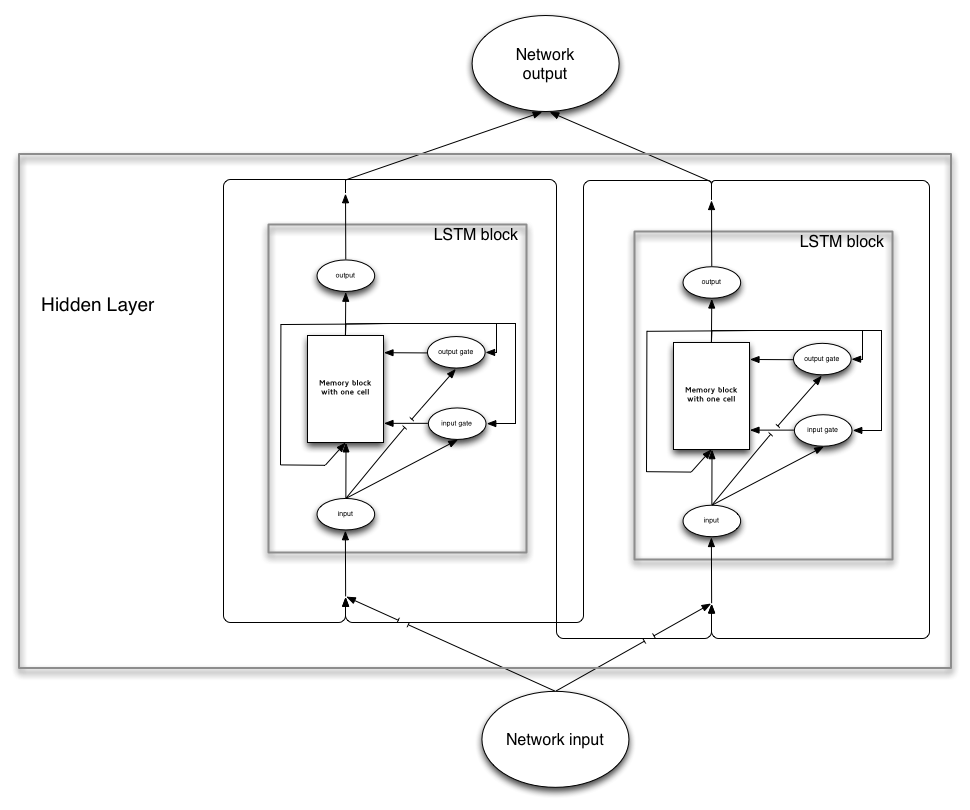
\includegraphics[height=.7\textheight]{figures/lstm2.png} \\
        \tiny from \url{http://stackoverflow.com/q/17454402/1163213}
        \end{center}
    \end{figure}
\end{frame}

\begin{frame}{Results}
    \begin{table}[H]
        \begin{center}
        \ra{1.2}
        % \footnotesize
        % \caption{Overview}
        \begin{tabular}{@{} lrrr @{}}
        \toprule
        % \multicolumn{4}{c}{\textbf{Random source}, $n=247$} \\
        {} & mean & std & mistake \\
        \midrule
        O'Connor  &     XXXXXXX &    XXXXXXX &    XXXXXXX \\
        Miller    &     XXXXXXX &    XXXXXXX &    XXXXXXX \\
        LSTM      &     XXXXXXX &    XXXXXXX &    XXXXXXX \\
        \bottomrule
        \end{tabular}
        \end{center}
    \end{table}
\end{frame}

\begin{frame}{Results}
    \begin{figure}
    \begin{center}
        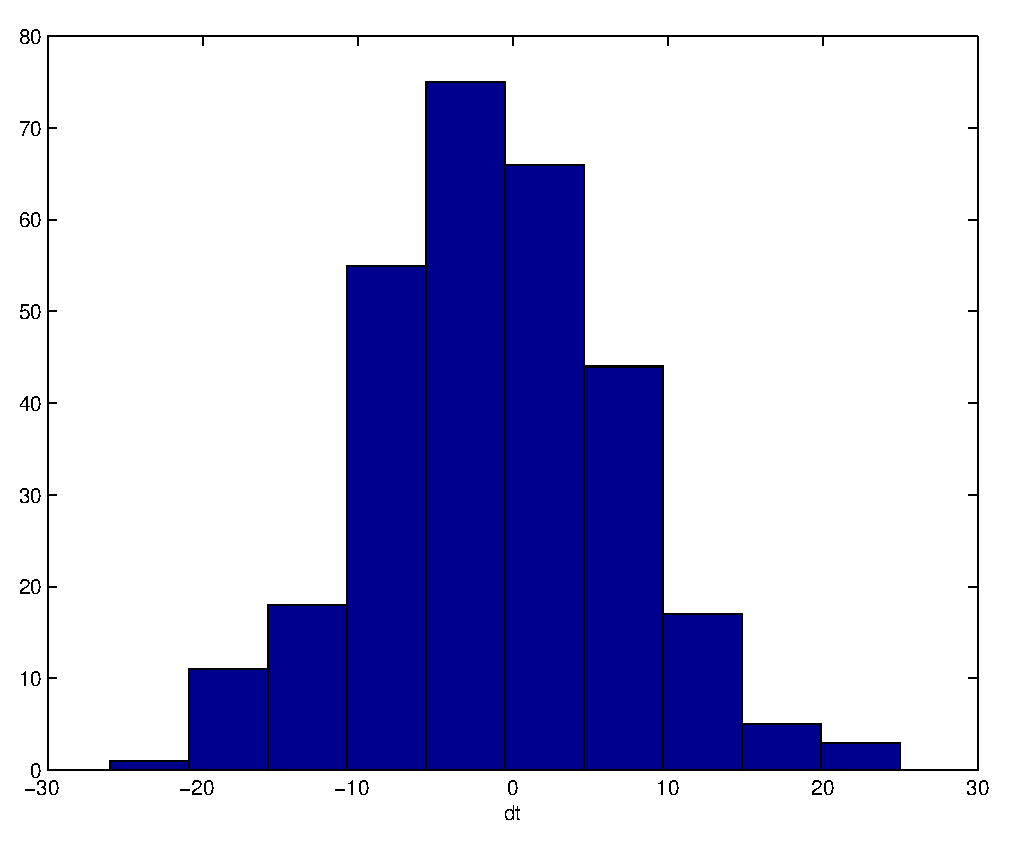
\includegraphics[width=0.75\textwidth]{figures/hist_miller.eps}
        \caption{Histogram Miller}
        \label{fig:hist_miller}
    \end{center}
    \end{figure}
\end{frame}

\begin{frame}{Q\&A}
    \Large
    \centering
    Thank you for your attention!
\end{frame}

\begin{frame}{Human Gait Cycle}
    \begin{figure}[H]
    \begin{center}
        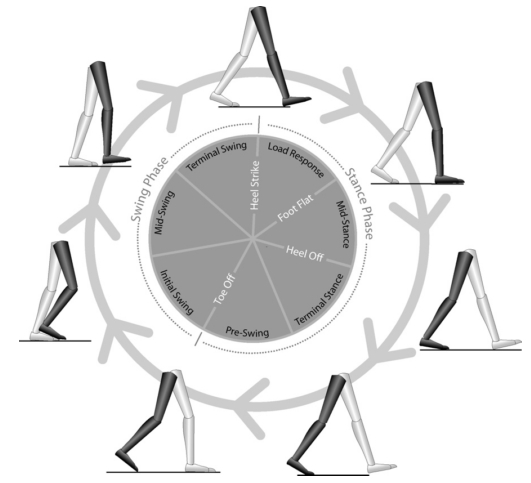
\includegraphics[height=.8\textheight]{figures/gait_events.jpg}
        \caption{Gait events [Rueterbories et al., 2010]}
        \label{fig:gait_events}
    \end{center}
    \end{figure}
\end{frame}

\begin{frame}{Lab setup (not our lab but similar)}
    \begin{figure}[H]
        \begin{center}
        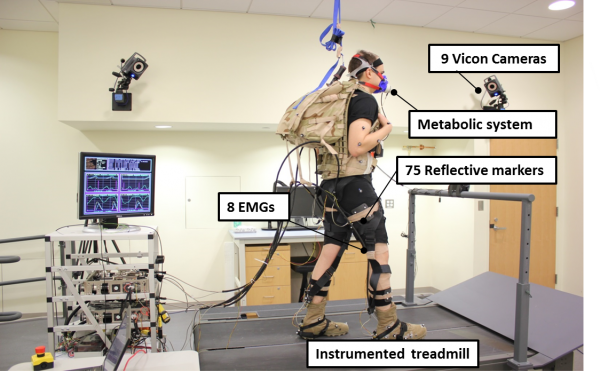
\includegraphics[height=.7\textheight]{figures/treadmill.png} \\
        \tiny from \url{http://biodesign.seas.harvard.edu/soft-exosuits}
        \end{center}
    \end{figure}
\end{frame}

\end{document}
